\section{Czym jest podtypowanie}
Koncept podtypowania jest dosyć intuicyjny. Wyobrazimy sobie na chwilę typy jako zbiory elementów należących do danego typu, wtedy podtyp to będzie podzbiorem naszego pierwotnego typu. Pozwala ono na wyrzucanie z typu wszystkich niepożądanych elementów z naszego typu pierwotnego. Dla przykładu wyobraźmy sobie, że piszemy funkcję wyszukiwania binarnego i jako jej argument chcielibyśmy otrzymać posortowaną listę. W tym celu właśnie możemy użyć podtypowania, wymuszając aby akceptowane były jedynie listy które spełniają predykat posortowania.
\begin{code}
\begin{minted}{coq}
Inductive sig (A : Type) (P : A -> Prop) : Type :=
    exist : forall x:A, P x -> sig P.
    
Record sig' (A : Type) (P : A -> Prop) : Type := exist' {
    proj1' : A;
    proj2' : P proj1';
}
\end{minted}
\caption{Dwie równoważne definicje podtypowania w Coqu.}
\label{sig}
\end{code}
Najbardziej ogólna definicja podtypowania \ref{sig} wymaga wykorzystania typów zależnych, które nie są dostępne w większości języków programowania, stąd też w większości języków programowania na programiście spoczywa obowiązek upewnienie się czy lista jest posortowana, gdyż ekspresywność języka jest zbyt uboga, aby zapisać takie wymagania. Coq w bibliotece standardowej \mintinline{coq}{Coq.Init.Specif} posiada zdefiniowane \mintinline{coq}{sig} wraz z notacją \mintinline{coq}{{a : A | P a}}, która ma przypominać matematyczny zapis $\{x \in A : P(x)\}$. Ta sama biblioteka posiada identyczną konstrukcje, gdzie jednak \mintinline{coq}{(P : A -> Prop)} zostało zamienione na \mintinline{coq}{(P : A -> Type)} jest to uogólniona definicja podtypowania, nazywana sigma typem.
\begin{code}
\begin{minted}{coq}
Inductive sigT (A:Type) (P:A -> Type) : Type :=
    existT : forall x:A, P x -> sigT P Q.
}
\end{minted}
\caption{Definicja definicja sigma typu z biblioteki standardowej Coqa.}
\end{code}
Jest to para zależna w której drugi element pary zależy do pierwszego. Posiada ona również zdefiniowaną notację \mintinline{coq}{{a : A & P}}, nawiązuje ona do tego \mintinline{coq}{a} jest zarówno typu \mintinline{coq}{A} jak i \mintinline{coq}{P}. 
\subsection{Dlaczego w ogóle wspominamy o podtypowaniu?}
Podtypowanie jest to dualna konstrukcja do typów ilorazowych o których mowa w tej pracy. Ten rozdział poświęcamy im z następującego powodu - Coq nie wspiera podtypowania. Nie możemy w żaden inny sposób niż aksjomatem wymusić równości dwóch różnych elementów danego typu. Używanie aksjomatów jest jednak nie praktyczne, gdyż niszczy obliczalność dowodu, a na dodatek bardzo łatwo takimi aksjomatami doprowadzić do sprzeczności w logice Coqa. Dlatego zastąpimy tutaj koncept typów ilorazowych konceptem podtypowania, który będzie wymuszać istnienie jedynie normalnych postaci danej klasy abstrakcji w naszym typie ilorazowym. 
\begin{code}
\begin{minted}{coq}
Record quotient {A: Type} {f: A -> A} (n: normalizing_function f) := {
  val: A;
  proof: val = f val
}.
\end{minted}
\caption{Definicja podtypu kanonicznych postaci względem funkcji normalizującej f.}
\end{code}
Pozwoli nam to na pracę jak na typach ilorazowych korzystając z ograniczonej liczby narzędzi, które dostarcza nam Coq. 
\section{Dualna? Co to oznacza?}
W poprzedniej sekcji wspomnieliśmy, że podtypowanie jest pojęciem dualnym do ilorazów, tu wyjaśnimy co to oznacza. Dualizm jest pojęciem ze świata teorii kategorii, aby zrozumieć tą sekcję wymagana jest bardzo podstawowa wiedza z tego zakresu. Jeśli ktoś jej natomiast nie posiada może spokojnie ją pominąć gdyż stanowi bardziej ciekawostkę niż integralną część tej pracy. Mówiąc formalnie jeśli $\sigma$ jest konstrukcją w teorii kategorii to konstrukcję dualną do niej $\sigma^{\textrm{op}}$ definiujemy poprzez: 
\begin{itemize}
    \item zamianę pojęć elementu początkowego i końcowego nawzajem,
    \item zmianę kolejności składania morfinizmów.
\end{itemize}
Mając to już za sobą możemy powiedzieć prostym językiem, że dualność polega na zmianie kierunku strzałek w naszej konstrukcji. 
\begin{figure}[!htp]
    \centering
    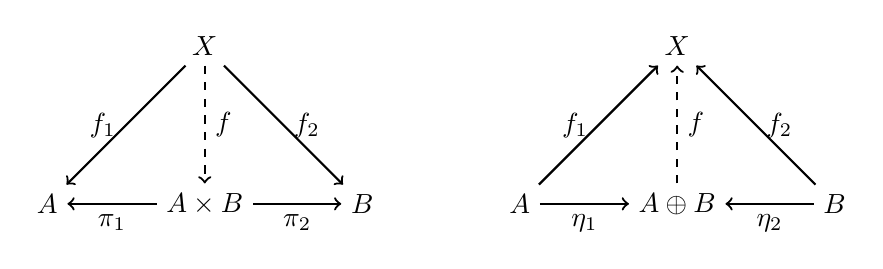
\begin{tikzpicture}[node/.style={circle, draw=black!60, very thick, minimum size=0.4}]
    %Nodes
    \node[] at (0, 0) (pA) {$A$};
    \node[] at (4, 0) (pB) {$B$};
    \node[] at (2, 2) (pX) {$X$};
    \node[] at (2, 0) (pS) {$A \times B$};
    
    \node[] at (6, 0) (cA) {$A$};
    \node[] at (10, 0) (cB) {$B$};
    \node[] at (8, 2) (cX) {$X$};
    \node[] at (8, 0) (cS) {$A \oplus B$};
    
    %Lines
    \draw[->, thick] (pS) -- (pA) node [below, midway] {$\pi_1$};
    \draw[->, thick] (pS) -- (pB) node [below, midway] {$\pi_2$};
    \draw[->, thick] (pX) -- (pA) node [left, midway] {$f_1$};
    \draw[->, thick] (pX) -- (pB) node [right, midway] {$f_2$};
    \draw[->, thick, dashed] (pX) -- (pS) node [right, midway] {$f$};
    
    \draw[->, thick] (cA) -- (cS) node [below, midway] {$\eta_1$};
    \draw[->, thick] (cB) -- (cS) node [below, midway] {$\eta_2$};
    \draw[->, thick] (cA) -- (cX) node [left, midway] {$f_1$};
    \draw[->, thick] (cB) -- (cX) node [right, midway] {$f_2$};
    \draw[->, thick, dashed] (cS) -- (cX) node [right, midway] {$f$};
    
    \end{tikzpicture}
    \caption{Przykład dwóch dualnych konstrukcji. Po lewej stronie widzimy produkt, a po prawej co-produkt. Oba diagramy komutują.}
    \label{fig:fourier_vis}
\end{figure}
Znając to pojęcie możemy zadać sobie pytanie gdzie w ilorazach i podtypowaniu występują jakieś strzałki, których kierunki mielibyśmy zamieniać? Występują mianowicie odpowiednio w pushoutach oraz pullbackach.
\subsection{Czym jest pushout?}
\begin{figure}[!htp]
    \centering
    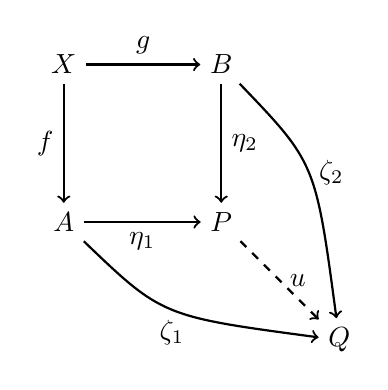
\begin{tikzpicture}[node/.style={circle, draw=black!60, very thick, minimum size=0.4}]
    %Nodes
    \node[] at (0, 0) (a) {$A$};
    \node[] at (2, 0) (p) {$P$};
    \node[] at (0, 2) (x) {$X$};
    \node[] at (2, 2) (b) {$B$};
    
    \node[] at (3.5, -1.5) (q) {$Q$};
    
    %Lines
    \draw[->, thick] (x) -- (a) node [left, midway] {$f$};
    \draw[->, thick] (x) -- (b) node [above, midway] {$g$};
    \draw[->, thick] (a) -- (p) node [below, midway] {$\eta_1$};
    \draw[->, thick] (b) -- (p) node [right, midway] {$\eta_2$};
    \draw[->, thick] (a) .. controls +(1.25, -1.2) .. (q) node [below, midway] {$\zeta_1$};
    \draw[->, thick] (b) .. controls +(1.2, -1.25) .. (q) node [right, midway] {$\zeta_2$};
    \draw[->, thick, dashed] (p) -- (q) node [right, midway] {$u$};
    
    \end{tikzpicture}
    \caption{Diagram definiujący pushout $P$. Diagram komutuje.}
    \label{fig:pushout_def}
\end{figure}
Na rysunku \ref{fig:pushout_def} możemy zobaczyć diagram definiujący pojęcie pushoutu. Widzimy, że powstaje on z pewnych dwóch morfinizmów $f:X \rightarrow A$ oraz $g:X \rightarrow B$. Ponieważ diagram ten komutuje wiemy, że $\eta_1 \circ f = \eta_2 \circ g$. Nasz pushout $P$ jest najlepszym takim obiektem dla którego diagram zachowuje tą własność. Najlepszy definiujemy jako, dla każdego innego obiektu (na diagramie $Q$), dla którego zewnętrzna część ($X, A, B, Q$) diagramu komutuje, istnieje unikatowy (dokładnie jeden) morfizm $u$ z $P$ do $Q$. Warto zaznaczyć, że nie dla każdych dwóch morfinizmów $f:X \rightarrow A$ oraz $g:X \rightarrow B$ istnieje pushout, jeśli jednak istnieje to jest unikatowy z dokładnością do unikatowego izomorfizmu.
\subsection{Przykład pushoutu w kategorii \emph{Set}}
W definicji pushoutu łatwo możemy zobaczyć morfizmy (strzałki), natomiast trudno odnaleźć ilorazy o których jest ta praca. Dużo łatwiej wyrobić swoją intuicję na bardziej przyziemnym przykładzie. Przenieśmy się w tym celu do kategorii \emph{Set}. Oznacza to, że nasze obiekty staną się zbiorami, a morfizmy (strzałki) funkcjami na zbiorach. Na rysunku \ref{fig:pushout_def} możemy zauważyć, że $A$, $B$ oraz $P$ tworzą coś na kształt co-produktu. Zatem warto zacząć definiowanie $P$ właśnie od $A \oplus B$. Wszystko byłoby wszystko dobrze gdyby nie to, że nasz diagram powinien komutować, a więc dla każdego $x \in X$ wiemy, że $\eta_1(f(x)) = \eta_2(g(x))$. Aby to zapewnić musimy utożsamić z sobą $f(x) \sim g(x)$, dla każdego $x \in X$. Dzięki podzieleniu przez tą relację zapewnimy sobie komutowane wewnętrznej części diagramu ($X, A, B, P$). Nie możemy jednak wziąć dowolnej relacji $\sim$ spełniającej ten warunek, gdyż musimy zapewnić istnienie funkcji $u$ do każdego innego zbioru dla którego ten diagram będzie komutował, oznacza to że musi istnieć surjekcja ze zbioru $P$ do $Q$. Z uwagi na komutowanie funkcja $u$ musi spełniać $u \circ \eta_1 = \zeta_1$ oraz $u \circ \eta_2 = \zeta_2$. Nasza relacja równoważności musi zatem być tą najdrobniejszą, aby spełnić ten warunek. Jeśli nasz pushout $P$ jest równy $(A \oplus B) / \sim$ diagram \ref{fig:pushout_def} będzie komutował.  Widzimy zatem, że pushout rzeczywiście ma jakiś związek z typami ilorazowymi, w których to $X$ definiuje które elementy zostaną z sobą utożsamione. 
\subsection{Sklejanie dwóch odcinków w okrąg, czyli pushout}
Rozważyliśmy bardziej przyziemny, lecz dojść abstrakcyjny przykład w kategorii \emph{Set}. Skonstruujmy nieco bardziej wizualny przykład, czyli w naszym przypadku okrąg na rysunku \ref{fig:pushout_circ_def}.
\begin{figure}[!htp]
    \centering
    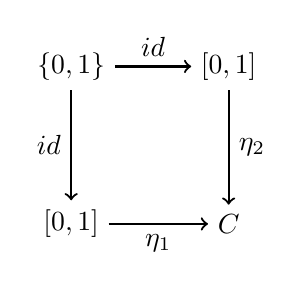
\begin{tikzpicture}[node/.style={circle, draw=black!60, very thick, minimum size=0.4}]
    %Nodes
    \node[] at (0, 0) (a) {$[0, 1]$};
    \node[] at (2, 0) (p) {$C$};
    \node[] at (0, 2) (x) {$\{0, 1\}$};
    \node[] at (2, 2) (b) {$[0, 1]$};
    
    %Lines
    \draw[->, thick] (x) -- (a) node [left, midway] {$id$};
    \draw[->, thick] (x) -- (b) node [above, midway] {$id$};
    \draw[->, thick] (a) -- (p) node [below, midway] {$\eta_1$};
    \draw[->, thick] (b) -- (p) node [right, midway] {$\eta_2$};;
    
    \end{tikzpicture}
    \caption{Diagram definiujący okrąg $C$ używając pushoutu}
    \label{fig:pushout_circ_def}
\end{figure}
Upewnijmy się, iż rzeczywiście $C$ jest topologicznym okręgiem. Wiemy, że aby diagram \ref{fig:pushout_circ_def} komutował $\eta_1(0) = \eta_2(0)$ oraz $\eta_1(1) = \eta_2(1)$. Skleiliśmy zatem z sobą te dwa punkty. Ponieważ $C$ musi być najlepszym obiektem dla którego diagram komutuje, to żadne inne elementy nie mogą być z sobą sklejone, a więc dla każdego $x \in (0, 1)$ wiemy, że $\eta_1(x) \not= \eta_2(x)$. Więc rzeczywiście stworzyliśmy okrąg, z dwóch odcinków oraz dwóch punktów sklejeń. Ta metoda uogólnia się do wyższych wymiarów. Mając dwie $n$-wymiarowe półkule, a następnie sklejając je w wzdłuż kuli ($n-1$)-wymiarowej otrzymamy kulę $n$-wymiarową. 
\subsection{Czym jest pullback?}
Wiedząc jak wygląda pushout oraz wiedząc, że pullback jest pojęciem do niego dualnym każdy powinien być w stanie narysować diagram go definiujący, możemy się mu przyjrzeć na rysunku \ref{fig:pullback_def}.
\begin{figure}[!htp]
    \centering
    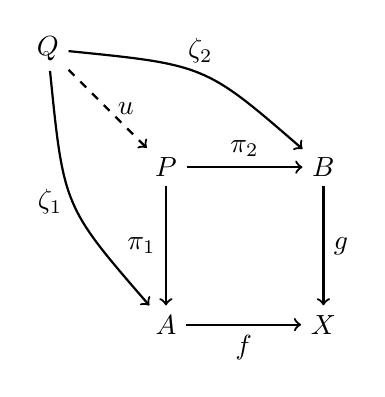
\begin{tikzpicture}[node/.style={circle, draw=black!60, very thick, minimum size=0.4}]
    %Nodes
    \node[] at (0, 0) (a) {$A$};
    \node[] at (0, 2) (p) {$P$};
    \node[] at (2, 0) (x) {$X$};
    \node[] at (2, 2) (b) {$B$};
    
    \node[] at (-1.5, 3.5) (q) {$Q$};
    
    %Lines
    \draw[->, thick] (a) -- (x) node [below, midway] {$f$};
    \draw[->, thick] (b) -- (x) node [right, midway] {$g$};
    \draw[->, thick] (p) -- (a) node [left, midway] {$\pi_1$};
    \draw[->, thick] (p) -- (b) node [above, midway] {$\pi_2$};
    \draw[->, thick] (q) .. controls +(0.2, -2) .. (a) node [left, midway] {$\zeta_1$};
    \draw[->, thick] (q) .. controls +(2, -0.2) .. (b) node [above, midway] {$\zeta_2$};
    \draw[->, thick, dashed] (q) -- (p) node [right, midway] {$u$};
    
    \end{tikzpicture}
    \caption{Diagram definiujący pullback $P$. Diagram komutuje.}
    \label{fig:pullback_def}
\end{figure}
Każdy pullback jest definiowany za pomocą dwóch morfizmów $f: A \rightarrow X$ oraz $g: B \rightarrow X$, które tworzą strukturę przypominającą co-produkt. Z komutacji wiemy, że $f \circ \pi_1 = g \circ \pi_2$. Podobnie jak w przypadku pushoutu, tu również aby $P$ był pullbackiem to musi być najlepszym obiektem, dla którego diagram komutuje. Oznacza to że dla każdego innego (na diagramie $Q$), dla którego zewnętrza część diagramu ($X, A, B, Q$) komutuje to istnieje unikatowy morfizm $u$ z $Q$ do $P$, który oczywiście zachowuje własność komutacji diagramu. Ponownie nie dla każdych dwóch morfizmów $f:A \rightarrow X$ oraz $g:B \rightarrow X$ istnieje pushout, jeśli jednak istnieje to jest unikatowy z dokładnością do unikatowego izomorfizmu.
\subsection{Przykład pullbacku w kategorii \emph{Set}}
Ponownie aby zobaczyć podtypowanie w zdefiniowanym powyżej pullbacku omawiane w tym rozdziale podtypowanie przeniesiemy się do prostszego świata kategorii $Set$, gdzie żyją zbiory oraz funkcje na zbiorach. Jak widzimy na diagramie \ref{fig:pullback_def} struktura $A$, $B$ oraz $P$ przypomina coś na kształt produktu. Zacznijmy więc definiowanie $P$ właśnie od $A \times B$. Wiemy jednak, że aby diagram komutował to dla każdego elementu $p \in P$ musi zachodzić własność $f (\pi_1 (p)) = g (\pi_2(p))$. Ponieważ wstępnie $P = A \times B$ to dla każdej pary $(a, b) \in A \times B$ zachodzi $f(a) = g(b)$. Wystarczy teraz wyrzucić wszystkie elementy nie spełniające tego warunki otrzymując ostatecznie $P = \{(a, b) \in A \times B : f(a) = g(b)\}$. Upewnijmy się jeszcze iż rzeczywiście to jest najlepszy wybór. Weźmy dowolny inny zbiór $Q$ wraz z funkcjami $\zeta_1$ oraz $\zeta_2$ dla którego zewnętrzny diagram \ref{fig:pullback_def} komutuje  i zdefiniujmy morfizm $u$ jako dla każdego $q \in Q$ mamy $u(q) = (\zeta_1(q), \zeta_2(q))$. Ponieważ funkcje $\pi_1$ i $\pi_2$ są zwykłymi projekcjami to własności $\zeta_1 = \pi_1 \circ u$ oraz $\zeta_2 = \pi_2 \circ u$ mamy za darmo, a cała reszta diagramu komutuje z względu na na komutowanie zewnętrznej części diagramu. Możemy na w tym miejscu zauważyć iż rzeczywiście pullback ma związek z podtypowaniem, poprzez wyrzucanie elementów które nie spełniają równości $f(a) = g(b)$.
\subsection{Pary liczb o tej samej parzystości, czyli pullback}
Mamy już za sobą definicję, oraz przykład w kategorii \emph{Set}. Możemy teraz przejść do stworzenia prostego podtypu, w tym przykładzie par liczb całkowitych o tej samej parzystości.  
\begin{figure}[!htp]
    \centering
    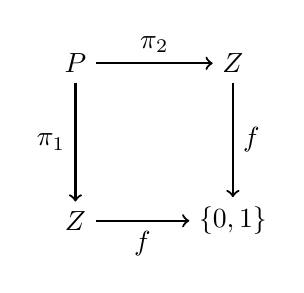
\begin{tikzpicture}[node/.style={circle, draw=black!60, very thick, minimum size=0.4}]
    %Nodes
    \node[] at (0, 0) (a) {$\mathbb{Z}$};
    \node[] at (0, 2) (p) {$P$};
    \node[] at (2, 0) (x) {$\{0, 1\}$};
    \node[] at (2, 2) (b) {$\mathbb{Z}$};
    
    %Lines
    \draw[->, thick] (a) -- (x) node [below, midway] {$f$};
    \draw[->, thick] (b) -- (x) node [right, midway] {$f$};
    \draw[->, thick] (p) -- (a) node [left, midway] {$\pi_1$};
    \draw[->, thick] (p) -- (b) node [above, midway] {$\pi_2$};;
    
    \end{tikzpicture}
    \caption{Diagram definiujący pary liczb całkowitych o tej samej parzystości $P$ używając pullbacku}
    \label{fig:pullback_pair_def}
\end{figure}
Na diagramie \ref{fig:pushout_circ_def} widzimy definicję pullbacku $P$ za pomocą morfizmu $f: \mathbb{Z} \rightarrow \{0, 1\}$, zdefiniowanej jako $f(n) = n \;\textrm{mod}\; 2$. Jak wiemy z poprzedniego przykładu $P = \{(n, m) \in \mathbb{Z} \times \mathbb{Z} : n \;\textrm{mod}\; 2 = m \;\textrm{mod}\; 2 \}$. A więc jest to zbiór to pary dwóch liczb całkowitych, które przystają do siebie molulo 2, czyli mówiąc inaczej mają tą samą parzystość.
\subsection{Konkluzja}
Jak więc zobaczyliśmy na poprzednich przykładach w teorii kategorii pushouty pozwalają nam na wyznaczenie obiektów, które utożsamiają z sobą pewne elementy względem pewnej relacji równoważności, generowanej przez morfizmy. Czyniąc je odpowiednikiem typów ilorazowych. Natomiast pullbacki pozwalają nam stworzyć obiekty z elementami które spełniają pewien zadany przez morfizmy warunek, czyniąc z nich odpowiedniki podtypów. Ponieważ te pojęcia są dualne co możemy zobaczyć na diagramach \ref{fig:pushout_def} oraz \ref{fig:pullback_def}, to możemy mówić o tych pojęciach jako dualnych do siebie nawzajem. 

\section{Unikatowość reprezentacji w podtypowaniu}
Podtypowanie w Coqu nie dostarcza nam jednak niestety tak przyjemnego interfejsu, jak moglibyśmy się spodziewać po matematycznym podejściu do tego konceptu. W teorii zbiorów jesteśmy przyzwyczajeni, że zapisów w stylu $8 \in \{x \in \mathbb{N}: \textrm{even}(x)\} $, w Coq natomiast zapis \mintinline{coq}{8 : {x : nat | even x}} powoduje konflikt typów, gdyż 8 jest typu \mintinline{coq}{nat}, a nie typu \mintinline{coq}{{x : nat | even x}}. Wynika to z  definicji \mintinline{coq}{sig}, gdzie \mintinline{coq}{sig} jest parą zależną w związku z tym, aby skonstruować element tego typu potrzebujemy dwóch składników, wartości oraz dowodu, że ta wartość spełnia spełnia wymagany przez podtypowanie predykat, w tym przypadku \mintinline{coq}{even}.

\begin{code}
\begin{minted}{coq}
Definition even (x: nat) : Prop := exists (t : nat), t + t = x.

Lemma eight_is_even : even 8.
Proof. red. exists 4. cbn. reflexivity. Qed.

Check (exist _ 8 eight_is_even) : {x : nat | even x}.
\end{minted}
\caption{Przykład elementu typu naturalnej liczby parzystej w Coqu}
\end{code}
Takie zdefiniowane podtypowanie rodzi pytanie o unikatowość reprezentacji. Cała koncepcja używania podtypowania do reprezentacji typów ilorazowych opiera się na tym, że będzie istnieć jedynie jeden element w postaci normalnej dla każdej klasy abstrakcji. Istnienie wielu takich elementów różniących się jedynie dowodem uniemożliwiłoby zastosowanie podtypowania do tego celu.
\begin{code}
\begin{minted}{coq}
Theorem uniqnes_of_representation : forall (A : Type) (P : A -> Prop) 
  (x y  : {a : A | P a}), proj1_sig x = proj1_sig y -> x = y.
\end{minted}
\caption{Twierdzenie mówiące o unikalności reprezentacji w podtypowaniu}
\label{uniqnes_of_representation}
\end{code}
Niestety twierdzenia \ref{uniqnes_of_representation} nie można udowodnić w Coq bez dodatkowych aksjomatów, natomiast wersja tego twierdzenia dla \mintinline{coq}{sigT} jest po prostu fałszywa. Pozostaje nam zatem zredukować oczekiwania, lub dodać dodatkowe założenia.
\subsection{Dodatkowe aksjomaty}
Pomimo iż w tej pracy unikamy używania dodatkowych założeń spoza Coq warto rozważyć jakie rezultaty dało by ich zastosowanie. 
\subsubsection{Aksjomat irrelewancji}
Jest to aksjomat mówiący o tym, że nie ma różnicy między dowodami tego samego twierdzenia. 
\begin{code}
\begin{minted}{coq}
Definition Irrelevance := forall (P: Prop) (x y: P), x = y.
\end{minted}
\caption{Definicja irrelewancji w Coqu}
\label{uniqnes_of_representation}
\end{code}
Jak możemy się domyśleć mając tak potężne narzędzie bez trudu możemy udowodnić twierdzenie \ref{uniqnes_of_representation}. 
\begin{code}
\begin{minted}{coq}
Theorem irrelevance_uniqnes : Irrelevance -> forall (A: Type) (P: A -> Prop)
  (x y: {z: A| P z}), proj1_sig x = proj1_sig y -> x = y.
Proof.
  intros Irr A P [x_v x_p] [y_v y_p] H.
  cbn in H; subst.
  apply eq_dep_eq_sig.
  specialize (Irr (P y_v) x_p y_p); subst.
  constructor.
Qed.
\end{minted}
\caption{Dowód unikalności reprezentacji używając irrelewancji w Coq}
\end{code}
Dodatkowo możemy udowodnić, że nasze unikatowość reprezentacji jest tak naprawę równoważna aksjomatowi irrelewacji dowodów.
\begin{code}
\begin{minted}{coq}
Theorem uniqnes_irrelevance : (forall (A: Type) (P: A -> Prop)
  (x y: {z: A| P z}), proj1_sig x = proj1_sig y -> x = y) -> Irrelevance.
Proof.
  intros Uniq P x y.
  specialize (Uniq unit (fun _ => P) (exist _ tt x) (exist _ tt y) eq_refl). 
  refine (eq_dep_eq_dec (A := unit) _ _).
  - intros. left. destruct x0, y0. reflexivity.
  - apply eq_sig_eq_dep. apply Uniq.
Qed.
\end{minted}
\caption{Dowód, że unikalności reprezentacji implikuje irrelewancję w Coq}
\end{code}
\subsubsection{Aksjomat K}
Aksjomat ten został wymyślony przez Habil Streicher w swojej pracy "Investigations Into Intensional Type Theory" \cite{Streicher}. My posłużymy się jego nieco zmodyfikowaną wersją (UIP - uniqueness of identity proofs), która lepiej oddaje konsekwencje jego użycia.
\begin{code}
\begin{minted}{coq}
Definition K := forall (A: Type) (x y: A) (p q: x = y), p = q.
\end{minted}
\caption{Aksjomat K w Coq}
\end{code}
Jest to nieco słabsza wersja aksjomatu irrelewancji, która mówi jedynie o irrelewanjci dowodów równości. Ma on pewną ciekawą konsekwencję, którą została opisana w \cite{Streicher}, a mianowicie pozwala on na zanurzenie równości na parach zależnych w zwykłą równość
\begin{code}
\begin{minted}{coq}
Theorem sig_jnjectivity : K -> forall (A : Type) (P : A -> Prop)
  (a : A) (p q : P a), exist P a p = exist P a q -> p = q.
\end{minted}
\caption{Twierdzenie o zanurzenie równości na parach zależnych w Coq}
\end{code}
Dowód tego twierdzenia pominiemy, lecz można go znaleźć w dodatku Stricher.v. Aksjomat K nie jest równoważny aksjomatowi irrelewacji \cite{gdzieś_dowód_tego} to nie można za jego pomocą udowodnić unikalności reprezentacji w ogólności. W przypadku jednak typów ilorazowych generowanych przez funkcję normalizującą, będziemy potrzebować jedynie predykatów równości.
\begin{code}
\begin{minted}{coq}
Inductive quotient {A: Type} {f: A -> A} (N: normalizing_function f) : Type :=
| existQ : forall x: A, x = f x -> quotient N.

Definition proj1Q {A: Type} {f: A -> A} {N: normalizing_function f} 
(x : quotient N) : A := let (a, _) := x in a.
\end{minted}
\caption{Definicja podtypu postaci kanoniczych generowanych przez funkcję normalizującą f, oraz projekcji dla niego w Coq}
\end{code}
Unikatowość reprezentacji dla tego typu można z łatwością udowodnić wykorzystując aksjomat K.
\begin{code}
\begin{minted}{coq}
Theorem uniqnes_quotient {A: Type} (f: A -> A) (N: normalizing_function f) 
    (q q': quotient N) : K -> (proj1Q q) = (proj1Q q') -> q = q'.
Proof.
  intros K H. 
  destruct q, q'. 
  cbn in *. subst. 
  destruct (K A x0 (f x0) e e0).
  reflexivity.
Qed.
\end{minted}
\caption{Dowód unikalności reprezentacji dla podtypu postaci kanoniczych generowanych przez funkcję normalizującą f w Coq}
\end{code}

Możemy w tym miejscu pójść nawet o krok dalej i zdefiniować, że wszystkie elementy będące w tej samej klasie abstrakcji mają unikalnego reprezentanta, przy założeniu aksjomatu K. Zaczniemy od dowodu że funkcja f rzeczywiście generuje relację równoważności \ref{equivalance_relation} \mintinline{coq}{norm_equiv}.
\begin{code}
\begin{minted}{coq}
Definition norm_equiv {A: Type} (f: A -> A) (N: normalizing_function f)
  (x y: A) : Prop := f x = f y.

Theorem norm_equiv_is_equivalance_relation (A: Type) (f: A -> A)
  (N:normalizing_function f) : equivalance_relation (norm_equiv f N).
Proof.
  unfold norm_equiv. apply equiv_proof.
  - intro x. reflexivity.
  - intros x y H. symmetry. assumption.
  - intros x y z H H0. destruct H, H0. reflexivity.
Qed. 
\end{minted}
\caption{Definicja relacji równoważności generowanej przez funkcję normalizującą w Coq}
\label{norm_equiv}
\end{code}
Mając już definicję jak wygląda ta relacja równoważności możemy przejść do właściwego dowodu.
\begin{code}
\begin{minted}{coq}
Theorem norm_equiv_quotient {A: Type} (f: A -> A) (N: normalizing_function f) 
  (q q': quotient N) : K -> norm_equiv f N (proj1Q q) (proj1Q q') -> q = q'.
Proof.
  intros K H. destruct q, q'.
  cbn in *. unfold norm_equiv in H. 
  assert (x = x0).
  - rewrite e, H, <- e0. reflexivity.
  - subst. destruct (K A x0 (f x0) e e0).
    reflexivity.
Qed.
\end{minted}
\caption{Dowód że wszystkie elementy w tej samej klasie abstrakcji mają wspólnego reprezentanta używając aksjomatu K}
\label{norm_equiv_quotient}
\end{code}
\subsubsection{Związek między tymi aksjomatami}
Jak już wspominaliśmy w ogólności aksjomat K jest szczególnym przypadkiem aksjomatu irrelewancji. Oznacza to że nie są one równoważne, jak ciekawostkę możemy powiedzić, że w świecie z ekstensjonalnością dowodów aksjomat K jest równoważny aksjomatowi irrelewancji.

\begin{code}
\begin{minted}{coq}
Definition Prop_ex : Prop := forall (P Q : Prop), (P <-> Q) -> P = Q.
\end{minted}
\caption{Predykat ekstensjonalności dowodów}
\label{Prop_ex}
\end{code}

\begin{code}
\begin{minted}{coq}
Theorem Irrelevance_K : Irrelevance -> K.
Proof.
  intros Irr A x y. apply Irr.
Qed. 
\end{minted}
\caption{Dowód że irrelewancja implikuje aksjomat K}
\label{Irrelevance_K}
\end{code}

\begin{code}
\begin{minted}{coq}
Theorem K_Irrelevance : Prop_ex -> K -> Irrelevance.
Proof.
  unfold Prop_ex, K, Irrelevance.
  intros Prop_ex K P x y. 
  assert (P = (P = True)).
  - apply Prop_ex. split.
    + intros z. rewrite (Prop_ex P True); trivial. split.
      * trivial.
      * intros _. assumption.
    + intros []. assumption.
  - revert x y. rewrite H. apply K.
Qed. 
\end{minted}
\caption{Dowód, że ekstensjonalność dowodów oraz aksjomat K implikuje irrelewancję}
\label{K_Irrelevance}
\end{code}

\subsection{Wykorzystując \mintinline{coq}{SProp}}
\mintinline{coq}{SProp} jest to uniwersum predykatów z definicyjną irrelewancją. Oznacza to że występuje w nim wbudowany aksjomat irrelewacji i wszystkie dowody tego samego typu można w nim przepisywać, bez dodatkowych założeń. Niestety jest to wciąż eksperymentalna funkcjonalność w Coqu i posiada bardzo ubogą bibliotekę standardową, która nie posiada nawet wbudowanej równości. Posiada natomiast kilka użytecznych konstrukcji:
\begin{description}
    \item[\mintinline{coq}{Box}] - jest to rekord, który pozwala opakować dowolne wyrażenie w \mintinline{coq}{SProp} i przenieść je do świata \mintinline{coq}{Prop},
    \item[\mintinline{coq}{Squash}] - jest to typ induktywny, które jest indeksowany wyrażeniem w \mintinline{coq}{Prop}. Pozwala na przeniesienie dowolnego predykatu do świata \mintinline{coq}{SProp}, co z uwagi na mają ilość konstrukcji w bibliotece standardowej jest bardzo użyteczne,
    \item[\mintinline{coq}{sEmpty}] - jest to odpowiednik \mintinline{coq}{False : Prop}. Posiada on regułę eliminacji z której wynika fałsz,
    \item[\mintinline{coq}{sUnit}] - jest to odpowiednik \mintinline{coq}{True : Prop}. Rrównież pozwala się wydostać z świata \mintinline{coq}{SProp}, za pomocą reguły eliminacji,
    \item[\mintinline{coq}{Ssig}] - jest to odpowiednik \mintinline{coq}{sig}. Ponieważ w tym świecie występuje definicyjna irrelewancja to w bibliotece standardowej wraz z nim otrzymujemy twierdzenie \mintinline{coq}{Spr1_inj}, które mówi o unikalności reprezentacji dla tego typu.
\end{description}
Aby pokazać, że używając podtypowania z \mintinline{coq}{Ssig} również mamy jednego reprezentanta dla klasy abstrakcji musimy zdefiniować najpierw równość oraz nasz typ postaci normalnych.
\begin{code}
\begin{minted}{coq}
Inductive Seq {A: Type} : A -> A -> SProp :=
| srefl : forall x: A, s_eq x x.
\end{minted}
\caption{Typ induktywny równości w \mintinline{coq}{SProp}}
\label{SEq}
\end{code}

\begin{code}
\begin{minted}{coq}
Definition Squotient {A: Type} {f: A->A} (N: normalzation f) : Type :=
  Ssig (fun x : A => Seq x (f x)).
\end{minted}
\caption{Typ postaci normalnych w \mintinline{coq}{SProp}}
\label{SEq}
\end{code}
Mając już podstawowe definicje możemy przejść do właściwego dowodu.

\begin{code}
\begin{minted}{coq}
Theorem only_one_repersentant {A: Type} (f: A -> A) (N: normalzation f) 
  (q q': Squotient N) : norm_equiv f N (Spr1 q) (Spr1 q') -> Seq q q'.
Proof.
  intro H. 
  destruct q, q'. cbn in *. 
  assert (E: Seq Spr1 Spr0).
  - unfold norm_equiv in H. destruct Spr2, Spr3.
    subst. constructor.
  - destruct E. constructor.
Qed.
\end{minted}
\caption{Dowód że wszystkie elementy w tej samej klasie abstrakcji mają wspólnego reprezentanta w \mintinline{coq}{Squotient}}
\label{norm_equiv_quotient}
\end{code}
Korzystanie z \mintinline{coq}{SProp} niesie z sobą jednak poważny problem jakim jest próba przeniesienia predykatu do \mintinline{coq}{Prop}. Gdybyśmy zamienili \mintinline{coq}{Seq} na zwykłą równość (\mintinline{coq}{=}), takim wypadku nie dałoby się udowadniać tego twierdzenia. Dowody w Coqu domyślnie są w uniwersum \mintinline{coq}{Prop} i to w nim chcielibyśmy mieć dowody dla naszych typów ilorazowych. Z uniwersum \mintinline{coq}{SProp} możemy się jedynie wydostać eliminując \mintinline{coq}{sEmpty} lub \mintinline{coq}{sUnit}, co nie gwarantuje możliwości wyprowadzenia analogicznego dowodu w \mintinline{coq}{Prop}.
\subsection{Homotopiczne podejście}
Co jeśli jednak nie chcemy używać dodatkowych aksjomatów i pracować w \mintinline{coq}{Prop}? W takiej sytuacji z ratunkiem przychodzi homotopiczna teoria typów. Jest to relatywnie nowa gałąź matematyki, która zajmuje się dowodami równości w różnych typach\cite{HoTT}. Homotopiczną interpretacją równości jest $\omega$-graf w którym punkty reprezentują elementy typów, a ścieżki dowody równości, ścieżki między ścieżkami dowody równości dowodów równości i tak dalej.
\subsubsection{$N$-typy}
Wprowadza ona różne poziomy uniwersów w których żyją typu w zależności od dowodów równości między nimi. Ich indeksowanie zaczynamy nie intuicyjnie od -2. Opiszmy istotne dla nas nas uniwersa:
\begin{description}
    \item{Contr} - jest to najniższe uniwersum, na poziomie minus dwa. Żyjące w nim typy mają dokładnie jeden element. Przykładem takiego typu jest \mintinline{coq}{unit}.
    \begin{code}
    \begin{minted}{coq}
     Class isContr (A: Type) := ContrBuilder {
       center : A;
       contr  : forall x: A, x = center
     }.
    \end{minted}
    \caption{Klasa typów żyjących w uniwersum Contr.}
    \label{isContr}
    \end{code}
    \item{HProp} - nie mylić z Coqowym \mintinline{coq}{Prop}. Dla typów z tego uniwersum wszystkie elementy są sobie równe. Przykładem mieszkańca tego uniwersum jest \mintinline{coq}{Empty}. Ponieważ nie ma on żadnych elementów, to w trywialny sposób wszystkie jego elementy są równe, ale brak elementów wyklucza bycie w Contr.
    \begin{code}
    \begin{minted}{coq}
     Class isHProp (P : Type) :=
       hProp : forall p q : P, p = q.
    \end{minted}
    \caption{Klasa typów żyjących w uniwersum HProp.}
    \label{isHProp}
    \end{code}
    \item{HSet} - tu również nie ma związku z Coqowym \mintinline{coq}{Set}. Jest to poziom zerowy hierarchii uniwersów. Typy żyjące w tym uniwersum charakteryzują się tym, że jeśli dwa elementy są sobie równe to istnieje tylko jeden dowód tego faktu. Można o tym myśleć jako, że dla tych typów prawdziwy jest aksjomat K. Przykładem takiego typu jest \mintinline{coq}{bool}. Dlaczego jednak ma on unikatowe dowody równości powiemy później. 
    \begin{code}
    \begin{minted}{coq}
     Class isHSet (X : Type) :=
       hSet : forall (x y : X) (p q : x = y), p = q.
    \end{minted}
    \caption{Klasa typów żyjących w uniwersum HSet.}
    \label{isHProp}
    \end{code}
\end{description}
Nie są to jedyne uniwersa. Na kolejnym poziomie żyją typy, dla których dowody równości, między dowodami równości są zawsze tym samym dowodem i tak dalej i tak dalej. Definicję dowolnego uniwersum możemy przyjrzeć się w \ref{IsNType}.
\begin{code}
\begin{minted}{coq}
Inductive universe_level : Type :=
| minus_two  : universe_level
| S_universe : universe_level -> universe_level.

Fixpoint isNType (n : universe_level) (A : Type) : Type :=
match n with
| minus_two => isContr A
| S_universe n' => forall x y: A, isNType n' (x = y)
end.
\end{minted}
\caption{Klasa typów żyjących w $n$-tym uniwersum.}
\label{IsNType}
\end{code}
Jak widzimy typy dowodów równości między elementami typu żyjącego w $(n+1)$-wszym uniwersum żyją na w $n$-tym uniwersum. Aby nabrać nieco więcej intuicji na temat poziomów uniwersów pozwolimy sobie na udowodnienie twierdzenia dotyczącego zawierania się uniwersów. 
\begin{code}
\begin{minted}{coq}
Lemma contr_bottom : forall A : Type, isContr A -> 
  forall x y : A, isContr (x = y).

Theorem NType_inclusion : forall A: Type, forall n : universe_level,
  isNType n A -> isNType (S_universe n) A.
Proof.
  intros A n; revert A.
  induction n; intros A H.
  - cbn in *; intros x y.
    apply contr_bottom; assumption.
  - simpl in *; intros x y.
    apply IHn.
    apply H.
Qed.
\end{minted}
\caption{Dowód, że typu żyjące w $n$-tym uniwersum, żyją też w $(n+1)$-pierwszym uniwersum.}
\label{NType_incusion}
\end{code}
Jak widzimy w twierdzeniu \ref{NType_incusion} każde kolejne uniwersum zwiera w sobie poprzednie. Dowód twierdzenia \mintinline{coq}{contr_bottom} pominiemy tutaj, lecz można się z nim zapoznać w dodatku HoTT.v. Wracając jednak to naszego podtypowania widzimy, że jak długo będziemy się zajmować typami, które żyją w uniwersum HSet, nie będziemy musieli się martwić o dowody równości między elementami tego typu. A więc doskonale nadają się one do bycia pierwotnymi typami dla naszych typów ilorazowych. Pozostaje tylko ustalić które typy należą do tego uniwersum, tu również z pomocą przychodzi homotopiczna teoria typów oraz twierdzenie Hedberg'ga \cite{hedberg_1998}.
\subsubsection{Typy z rozstrzygalną równością}
Na początku warto definiować czym jest rozstrzygalna równość. Dla każdego typu z rozstrzygalną równością istnieje obliczalna (taka która można napisać w Coqu) funkcja która określa czy dwa elementy danego typu są tym samym elementem, czy też nie. 
\begin{code}
\begin{minted}{coq}
Class Decidable (A : Type) :=
  dec : A + (A -> False).

Class DecidableEq (A : Type) :=
  dec_eq : forall x y: A, Decidable (x = y).
\end{minted}
\caption{Definicja rozstrzygalności, oraz rozstrzygalnej równości.}
\label{NType_incusion}
\end{code}
Dobrym przykładem rozstrzygalnego typu jest \mintinline{coq}{bool}. Natomiast rozstrzygalnej równości nie ma na przykład typ funkcji \mintinline{coq}{nat -> nat}. Wspomniane wcześniej twierdzenie Hedberg'ga \cite{hedberg_1998} mówi o tym, że każdy typ z rozstrzygalną równością żyje w uniwersum \emph{HSet}. Dowód zaczniemy od zdefiniowania klasy typów sprowadzalnych.
\begin{code}
\begin{minted}{coq}
Class Collapsible (A : Type) :={ 
  collapse        : A -> A ;
  wconst_collapse : forall x y: A, collapse x = collapse y;
}.
\end{minted}
\caption{Definicja sprowadzalności.}
\label{Collapsible}
\end{code}
Pokażemy, że każdy typ rozstrzygalny jest sprowadzalny \ref{dec_is_collaps}.
\begin{code}
\begin{minted}{coq}
Theorem dec_is_collaps : forall A : Type, Decidable A -> Collapsible A.
Proof.
  intros A eq. destruct eq.
  - exists (fun x => a). intros x y. reflexivity.
  - exists (fun x => x); intros x y.
    exfalso; apply f; assumption.
Qed.
\end{minted}
\caption{Dowód, że każdy typ rozstrzygalny jest sprowadzalny.}
\label{dec_is_collaps}
\end{code}
Szczególnym przypadkiem są więc typy z rozstrzygalną równością, które mają sprowadzalne dowody równości (ścieżki) \ref{PathCollapsible}.
\begin{code}
\begin{minted}{coq}
Class PathCollapsible (A : Type) :=
  path_coll : forall (x y : A), Collapsible (x = y).

Theorem eq_dec_is_path_collaps : forall A : Type, DecidableEq A -> PathCollapsible A.
Proof.
  intros A dec x y. apply dec_is_collaps. apply dec.
Qed.
\end{minted}
\caption{Definicja wraz z dowodem, że każdy typ z rozstrzygalną równością ma sprowadzalne ścieżki.}
\label{PathCollapsible}
\end{code}
Mając już zdefiniowane sprowadzalne ścieżki, potrzebujemy jeszcze szybkiego dowodu, na temat pętli ścieżek \ref{loop_eq}.
\begin{code}
\begin{minted}{coq}
Lemma loop_eq : forall A: Type, forall x y: A, forall p: x = y, 
  eq_refl = eq_trans (eq_sym p) p.
Proof.
  intros A x y []. cbn. reflexivity.
Qed.
\end{minted}
\caption{Dowód, że każda pętla z ścieżek jest \mintinline{coq}{eq_refl}.}
\label{loop_eq}
\end{code}
Mając to już za sobą możemy przejść do właściwego dowodu, że dowolny typ z sprawdzalnymi ścieżkami jest \emph{HSet}'em \ref{path_collaps_is_hset}.
\begin{code}
\begin{minted}{coq}
Theorem path_collaps_is_hset (A : Type) : PathCollapsible A -> isHSet A.
Proof.
  unfold isHSet, PathCollapsible; intros C x y.
  cut (forall e: x=y, e = eq_trans (eq_sym(collapse(eq_refl x))) (collapse e)).
  - intros H p q. 
    rewrite (H q), (H p), (wconst_collapse p q).
    reflexivity.
  - intros []. apply loop_eq.
Qed.
\end{minted}
\caption{Dowód, że każdy typ z sprowadzalnymi ścieżkami jest HSet'em.}
\label{path_collaps_is_hset}
\end{code}
Jak więc widzimy każdy typ z rozstrzygalną równością ma tylko jeden dowód równości między dowolną parą równych sobie elementów. Oznacza to, że bez żadnych dodatkowych aksjomatów możemy udowodnić unikalność reprezentacji dla naszych typów ilorazowych, które mają rozstrzygalny typ pierwotny. Z uwagi na to, iż zdefiniowanie nie trywialnej funkcji normalizującej na typie bez rozstrzygalnej równości jest prawie nie możliwe, typy z rozstrzygalną równością wystarczą nam w tym rozdziale.
\subsubsection{Równość między parami zależnymi}
Podtypowanie w Coqu opiera się na parach zależnych, warto się przyjrzeć w jaki sposób wygląda równość między takimi parami. W przypadku zwykłych par sprawa jest prosta.
\begin{code}
\begin{minted}{coq}
Theorem pair_eq : forall (A B: Type) (a x : A) (b y : B),
  (a, b) = (x, y) -> a = x /\ b = y.
Proof.
  intros. inversion H. split; trivial.
Qed.
\end{minted}
\caption{Charakterystyka równości dla par.}
\label{pair_eq}
\end{code}
Jeśli jednak spróbujemy napisać to samo dla par zależnych otrzymamy błąd wynikający z niezgodności typów dowodów, nawet jeśli pozbędziemy się go ustalając wspólną pierwszą pozycję w parze to nie uda nam się udowodnić iż równość pary implikuje równość drugich elementów tych par, gdyż taka zależność implikowałaby aksjomat K \cite{Streicher}. Aby zrozumieć równość par zależnych musimy najpierw zdefiniować transport.
\begin{code}
\begin{minted}{coq}
Definition transport {A: Type} {x y: A} {P: A -> Type} (path: x = y) 
  (q : P x) : P y :=
match path with
| eq_refl => q
end.
\end{minted}
\caption{Definicja transportu.}
\label{transport}
\end{code}
Transport pozwala na przeniesienie typu \mintinline{coq}{q : P x} wzdłuż ścieżki \mintinline{coq}{path : x = y} do nowego typu \mintinline{coq}{P y}. Pozwala on pozbyć się problemu niezgodności typów w charakterystyce równości na parach zależnych.
\begin{code}
\begin{minted}{coq}
Theorem dep_pair_eq : forall (A: Type) (P: A->Type) (x y: A) (p: P x) (q: P y),
  existT P x p = existT P y q -> exists e: x = y, transport e p = q.
Proof.
  intros A P x y p q H. inversion H.
  exists eq_refl. cbn. trivial.
Qed.
\end{minted}
\caption{Charakterystyka równości dla par zależnych.}
\label{dep_pair_eq}
\end{code}
Jak więc wynika z twierdzenia \ref{dep_pair_eq} równość par zależnych składa się z równości na pierwszych elementów, oraz na równości drugich elementów przetransportowanej wzdłuż pierwszej równości.
